\documentclass{beamer}

\usepackage[utf8]{inputenc}
\usepackage{subfigure}

\title{Multimodal Corpora}
\subtitle{A brief summary with three examples}
\author{Tuan Pham Minh, Nils Harder, Tilman Krokotsch}
\date{January 17, 2017}

\begin{document}

	\beamertemplatenavigationsymbolsempty
	\setbeamercolor{title}{fg=black}
	\setbeamercolor{frametitle}{fg=black}
	\setbeamercolor{local structure}{fg=black}
	
	\setcounter{tocdepth}{1}

	\maketitle
	
	\begin{frame}
		\tableofcontents
	\end{frame}
	
	\section{BAS SmartKom Corpus} 	
	
	\section{The CALLAS Expressivity Corpus}	
	
	\section{The Bielefeld Speech and Gesture Alignment Corpus}
		\subsection{Recording Scenario}
			\begin{frame}{The Bielefeld Speech and Gesture Alignment Corpus}{Recording Scenario}
				\begin{figure}
					\subfigure{
						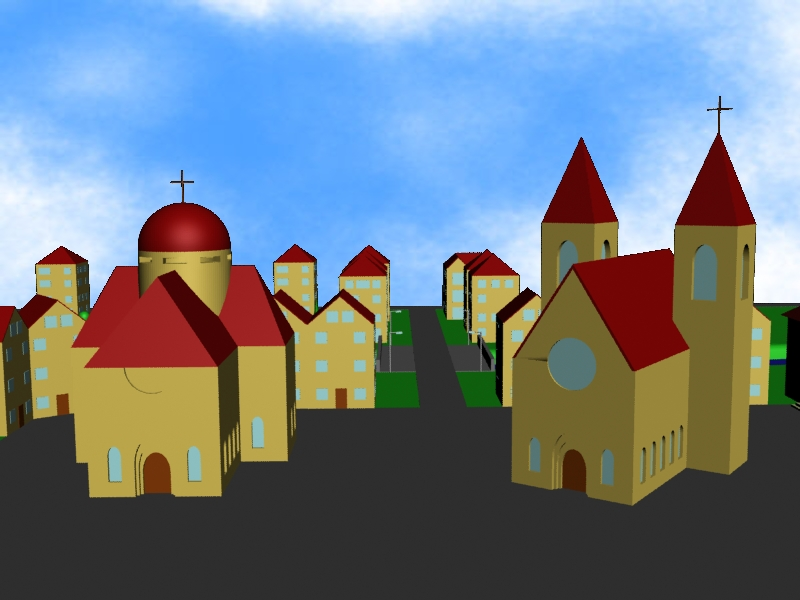
\includegraphics[width=0.48\textwidth]{Scenario}
					}
					\subfigure{
						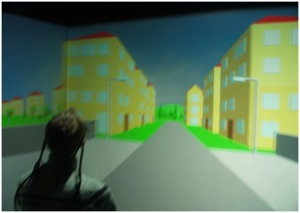
\includegraphics[width=0.48\textwidth]{Scenario_2}
					}
				\end{figure}
			\end{frame}
		
		\subsection{Recorded Data}
			
				\begin{frame}{The Bielefeld Speech and Gesture Alignment Corpus}{Primary Data}
					\begin{figure}
						\subfigure{
								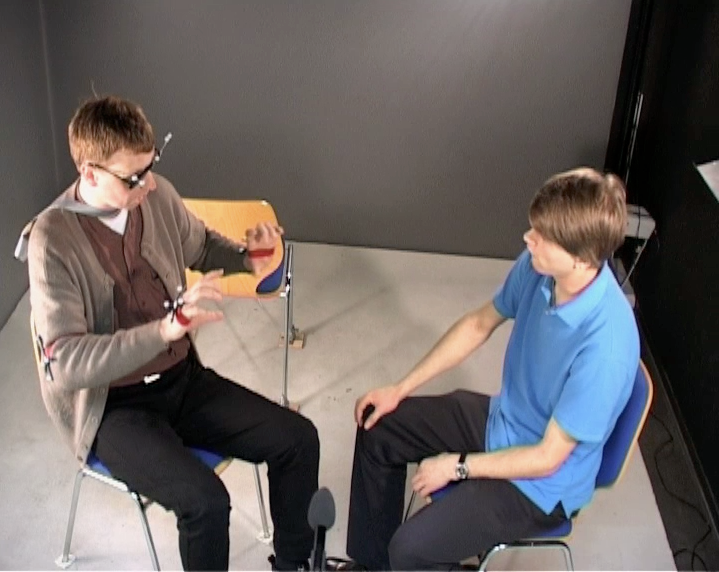
\includegraphics[width=0.4\textwidth]{Primary_1}
						}
						\subtable{
							\resizebox{0.5\textwidth}{!}{%
							\begin{tabular}{|l|c|}
								\hline 
								\textbf{Specification} & \textbf{Value} \\ 
								\hline 
								Number of dialogs & 25 \\ 
								\hline 
								Video time & 280 minutes \\ 
								\hline 
								Video specification & 720x576, 25fps  \\ 
								\hline 
								Video codec & H.264  \\ 
								\hline 
								Video feeds & 3 \\ 
								\hline 
								Audio feeds & 1 \\ 
								\hline
							\end{tabular} 
							}
						}
					\end{figure}
				\end{frame}
			
				\begin{frame}{The Bielefeld Speech and Gesture Alignment Corpus}{Secondary Data}
					\begin{figure}
					\subfigure{
						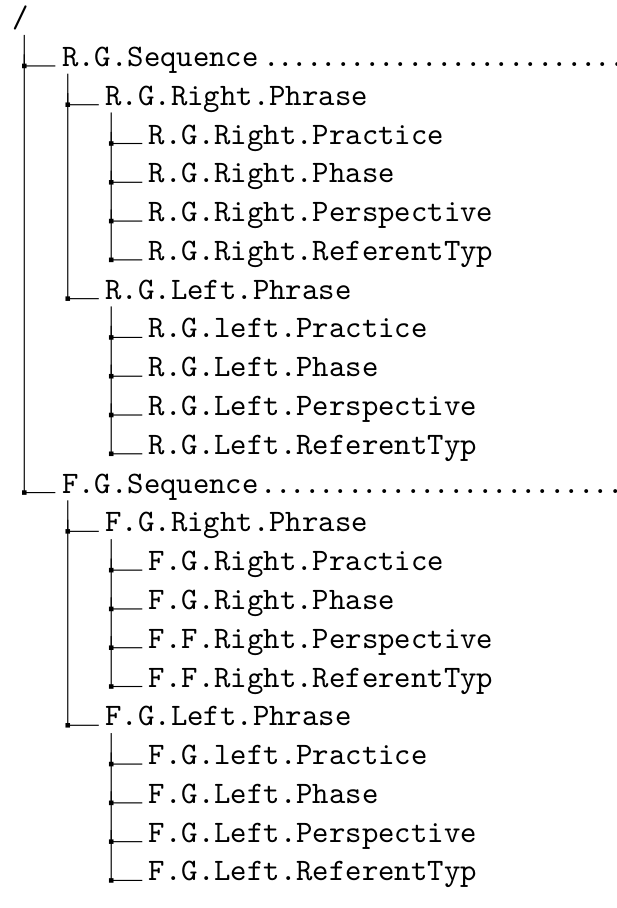
\includegraphics[width=0.45\textwidth]{Annotation_Scheme}
					}
					\subfigure{
						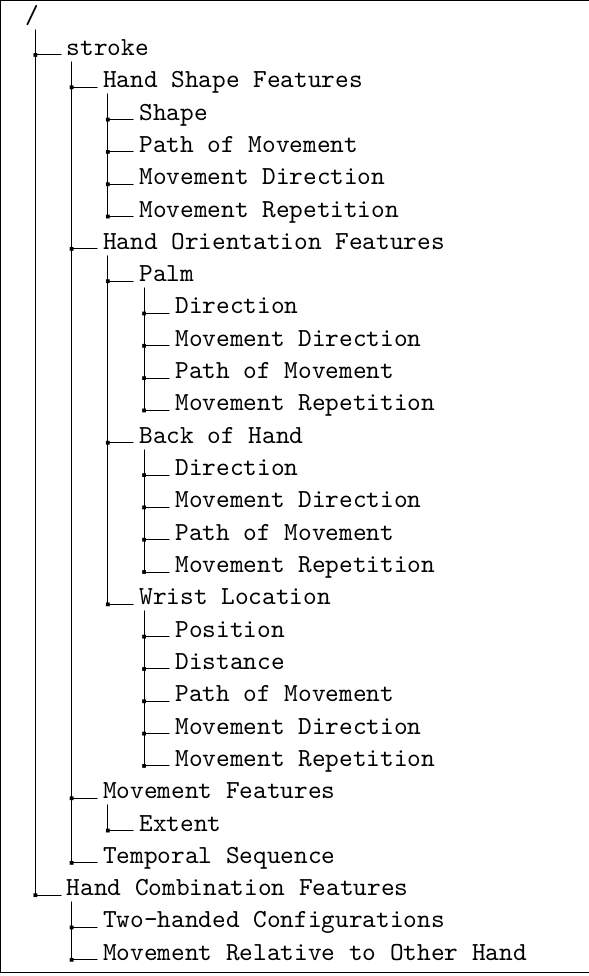
\includegraphics[width=0.45\textwidth]{Annotation_Scheme_2}
					}
				\end{figure}
				\end{frame}
			
				\begin{frame}{The Bielefeld Speech and Gesture Alignment Corpus}{Secondary Data}
					\begin{table}
						\center
						\begin{tabular}{|l|c|}
							\hline
							\textbf{Specification} & \textbf{Value} \\ 
							\hline 
							Words & 39,435 \\ 
							\hline 
							Iconic/Deictic gestures & 4961 \\ 
							\hline 
							Discourse gestures & approx. 1000 \\ 
							\hline 
						\end{tabular}
					\end{table}
				\end{frame}
		
		\subsection{Application}
			\begin{frame}{The Bielefeld Speech and Gesture Alignment Corpus}{Application}
				\center
						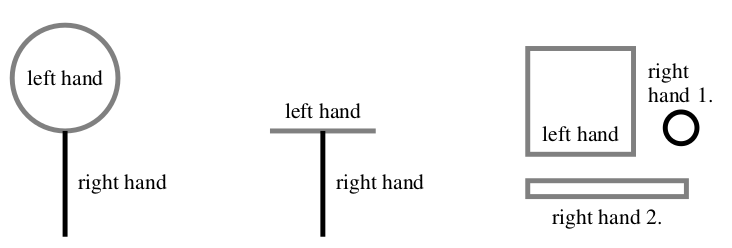
\includegraphics[width=0.7\textwidth]{Types}
						\vspace*{1cm}
						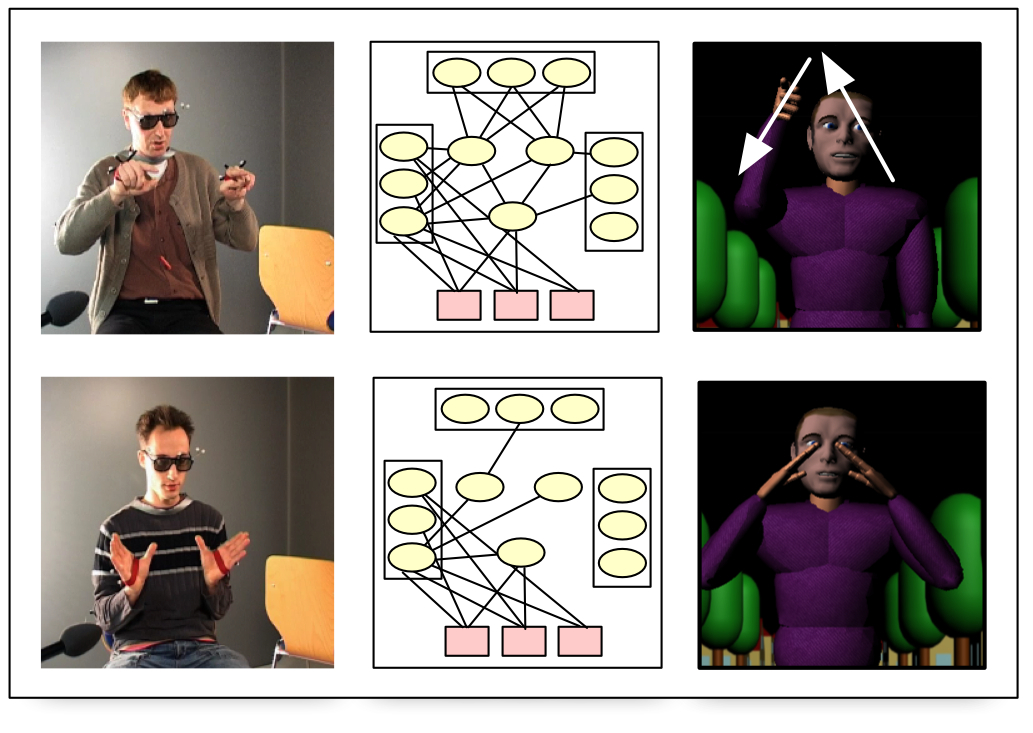
\includegraphics[width=0.6\textwidth]{Bayes}
			\end{frame}	
	
	\section{Sources}
		\begin{frame}{Sources}
			\bibliographystyle{IEEEtran}
			\nocite{Bielefeld2010}
			\nocite{Bielefeld2013}
			\nocite{Bergmann2014}
			\nocite{BAS2014}

  			\small\bibliography{../thebib}
		\end{frame}
	
\end{document}